\newpage
\section{Configuration Management Implementation}\label{sec:configuration-management-implementation}

This section describes the implementation of the three concepts,
~\textthreequartersemdash~\textit{static}, \textit{runtime} and \textbf{resource configuration}~\textthreequartersemdash~
introduced in the concepts section of the thesis~\ref{sec:configuration-management-concepts}
and specified by the according milestone~\ref{subsubsec:milestone-configuration-management}.


\subsection{NSAK Configuration Management}\label{subsec:nsak-configuration-management}

The \gls{NSAK} configuration is split into two distinct layers: a static layer that resolves fixed paths at import time, and a mutable runtime layer that is persisted to disk and loaded on every invocation.

\subsubsection{Static Configuration}\label{subsubsec:static-configuration}

The static configuration is defined in \mintinline{bash}{src/nsak/core/settings.py} and shown in listing~\ref{lst:nsak-settings}.
It derives all relevant paths from a single \mintinline{bash}{BASE_PATH}, which is either supplied via the \mintinline{bash}{NSAK_BASE_PATH} environment variable or resolved automatically to the repository root at import time.
\mintinline{bash}{RUN_PATH} points to the \mintinline{bash}{run/} directory where runtime data such as the persisted config is stored, and \mintinline{bash}{LIBRARY_PATHS} holds the set of directories that are searched for resource libraries.
Overriding \mintinline{bash}{NSAK_BASE_PATH} is the primary mechanism to run \gls{NSAK} from a different base directory, e.g.\ inside a \gls{Docker} container or during automated testing.


\subsubsection{Runtime Configuration}\label{subsubsec:runtime-configuration}

The runtime configuration is defined as the \enquote{Config} dataclass in \mintinline{bash}{src/nsak/core/configuration/configuration.py} and holds all state that can change during normal operation, currently the \mintinline{bash}{debug} flag and the active \enquote{Device}.
It is persisted as a \gls{YAML} file at \mintinline{bash}{run/config.yaml} and loaded on every \gls{CLI} invocation.

To avoid loading the configuration on import, the module-level \mintinline{bash}{config} object is wrapped in a \mintinline{python}{lazy_object_proxy.Proxy}.
The proxy defers the actual \mintinline{python}{Config.load()} call until the object is first accessed.
Since the root \gls{CLI} group imports \mintinline{bash}{config} on every command invocation as displayed in listing~\ref{lst:nsak-cli-init}, this ensures the configuration is always initialized before any command logic runs.
If \mintinline{bash}{run/config.yaml} does not yet exist, \mintinline{python}{Config.init()} is called automatically to create a default configuration and write it to disk, eliminating the need for manual setup on first run.


Mutations to the runtime configuration always follow the same pattern: a manager method (e.g.~\mintinline{bash}{DeviceManager.load()}) updates the relevant field on the \mintinline{bash}{config} object and calls \mintinline{python}{config.save()} to persist the change.
Custom \gls{YAML} representers are registered for \mintinline{python}{IPInterface} and \mintinline{python}{PosixPath} so that these types are serialised as plain strings rather than Python-specific tags.
Listing~\ref{lst:nsak-config-yaml} shows an example of the persisted \mintinline{bash}{run/config.yaml} after loading the \mintinline{bash}{bananapi_r4} device.



\subsection{Device Configuration Management}\label{subsec:device-configuration-management}

In the context of \enquote{Project 2}\ref{sec:predecessor-project-project-2}, this resource type was already defined conceptually, and the~\gls{BananaPI R4} was added as an example in the library under \mintinline{bash}{lib/devices/bananapi_r4/}.
But the resource type was not actually added to the \gls{NSAK} core, and to manage device configurations, we need to implement the Device resource type first.

\subsubsection{Create New Device Resource Type}\label{subsubsec:create-new-device-resource-type}

Similar to the other resource types, a \gls{YAML} specification for defining devices in the library and multiple classes for representing and managing devices in the core are required.
Because the existing resource \gls{YAML} specifications do not allow merging \gls{YAML} files,
this implementation proposes a new base structure that fulfills this trait.
Section~\ref{subsubsec:refactor-existing-resources} describes the necessary changes to the existing \gls{YAML} specifications.
The listing~\ref{lst:device-resource-yaml-specification} shows the initial specification for a device resource, which will get extended later on with a section for configuration management.


In the table~\ref{tab:device-resource-classes} below, the required Python classes are listed and described.
The classes will be located under \mintinline{bash}{src/nsak/core/device} within their respective files.

\begin{table}[h]
    \centering
    \begin{tabularx}{\textwidth}{llX}
        \hline
        \textbf{Class} & \textbf{File Name} & \textbf{Description} \\
        \hline
        Device & device.py & Dataclass representing a device resource at runtime, closely reflecting the \gls{YAML} specification. \\
        DeviceLoader & device\_loader.py & Loads and returns Device instances from the resource library. \\
        DeviceManager & device\_manager.py & Implements business logic and exposes an \gls{API} for use by the \gls{CLI}. \\
        \hline
    \end{tabularx}
    \caption{Device Resource Classes}
    \label{tab:device-resource-classes}
\end{table}

In \enquote{Project 2}\ref{sec:predecessor-project-project-2}, it became already clear that the described classes share a lot of boilerplate code between each other.
For this reason, the base classes described in~\ref{tab:device-resource-classes} were added to eliminate duplicated logic, thereby improving compliance with the \gls{DRY} principles.
The classes will be located under \mintinline{bash}{src/nsak/core/resource} within their respective files and the adoption of the existing classes is described in section~\ref{subsubsec:refactor-existing-resources}.

\begin{table}[h]
    \centering
    \begin{tabularx}{\textwidth}{llX}
        \hline
        \textbf{Class} & \textbf{File Name} & \textbf{Description} \\
        \hline
        Resource & resource.py & Base class for all resources: Scenario, Drill, Environment and Device. \\
        ResourceLoader & resource\_loader.py & Base class which handles searching and loading resources from the filesystem. \\
        ResourceManager & resource\_manager.py & Base class which defines common methods for all resource manager classes. \\
        \hline
    \end{tabularx}
    \caption{Resource Python Classes}
    \label{tab:resource-base-classes}
\end{table}

To complete the integration of the device resource, the new functionality must be exposed via \gls{CLI}.
The available bash commands are shown in the listing~\ref{lst:nsak-cli-list-devices}.



\subsubsection{Device Configuration Management Implementation}\label{subsubsec:device-configuration-management-implementation}

To allow a device to expose its configuration options, the \gls{YAML} specification needs to be extended accordingly.
For now, the focus is only on network configuration, as this is the most important information for the scenarios and drills.
The specification was designed so that other sections can be added later.
The excerpt~\ref{lst:device-resource-configuration-yaml-specification} shows the specification for the configuration section of the device resource \gls{YAML}.


The code snippet, located under \mintinline{bash}{src/nsak/core/device/device_loader.py}~\ref{lst:device-loader-configuration-parsing} shows how the \gls{YAML} configuration gets parsed to the respective datastructures defined in~\mintinline{bash}{src/nsak/core/network/configuration.py} and~\mintinline{bash}{src/nsak/core/device/device.py}~\ref{lst:device-configuration-datastructures}.


The referenced listing shows the newly available \gls{CLI} commands for managing device configurations~\ref{lst:device-configuration-cli-management}:


\subsubsection{Refactor Existing Resources}\label{subsubsec:refactor-existing-resources}

The implementation of the device resource~\ref{subsec:device-configuration-management} introduced an improved base structure for the resource \gls{YAML} specifications and
three base classes which are abstracting the common structure and functionality.
This section describes the resulting changes in the existing code and resource \gls{YAML} specifications.

As already stated in section~\ref{subsubsec:device-configuration-management-implementation} all resource type specific classes were refactored to inherit from their respective base classes
as described in table~\ref{tab:device-resource-classes}.
With the example of the \mintinline{bash}{EnvironmentLoader}, the diff below~\ref{fig:environment-loader-base-class-refactor-diff} illustrates how the abstraction of common properties and methods allows for the removal of a lot of boilerplate code.

\begin{figure}[H]
    \centering
    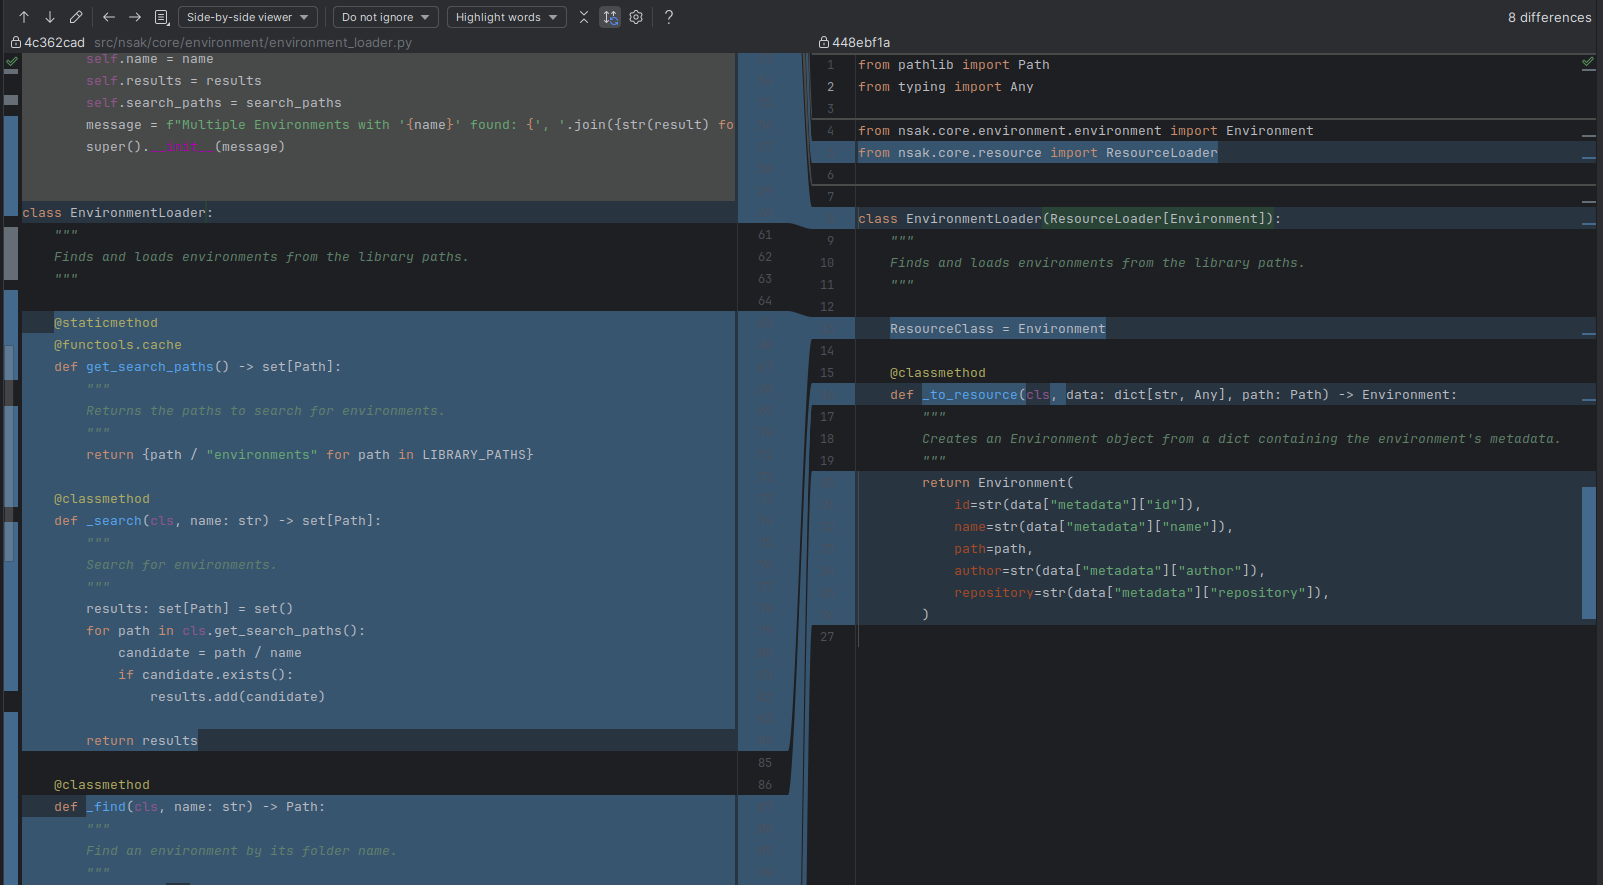
\includegraphics[width=1.0\linewidth]{../assets/screenshots/configuration_management/environment_loader_base_class_refactoring_diff}
    \caption{EnvironmentLoader Base Class Refactoring Diff}
    \label{fig:environment-loader-base-class-refactor-diff}
\end{figure}

The structure of all resources was aligned by nesting the resource under their respective resource type key (\mintinline{bash}{scenarios}, \mintinline{bash}{drills}, \mintinline{bash}{environments}, and \mintinline{bash}{devices}),
so that we could merge all \gls{YAML} resource files into a single library data structure without key conflicts.
In the \gls{YAML} specification~\ref{lst:mergeable-resource-yaml-specification}, the new base structure derived from the device resource~\ref{subsubsec:create-new-device-resource-type} is illustrated.
All existing resource \gls{YAML} files in the library were adjusted accordingly, and thanks to the introduction of the \mintinline{bash}{ResourceLoader} base class,
the required adjustments in the code were minimal.


\subsection{Scenario \& Drill Configuration Management}\label{subsec:drill-configuration-management}

Both the scenario and drill resource types were already fully implemented in \enquote{Project 2}\ref{sec:predecessor-project-project-2}.
Their \gls{YAML} specifications already contained an \mintinline{bash}{interface} section describing argument and return types, but this information was purely documentary and had no effect at runtime.

As part of this project, the \mintinline{bash}{interface.arguments} section was extended~\ref{lst:updated-interface-specification} so that each argument carries an explicit \mintinline{bash}{type} annotation and an optional \mintinline{bash}{default} value.


The \gls{CLI} reads these annotations at runtime to generate typed command options for each drill and scenario automatically, without requiring any additional handwritten code.
The \mintinline{bash}{discover_hosts} drill in listing~\ref{lst:discover-hosts-drill-yaml} illustrates this: its single \mintinline{bash}{interface} argument of type \mintinline{bash}{str} is translated directly into a \mintinline{bash}{--interface} option on the generated \gls{CLI} command.

Scenarios follow the same \mintinline{bash}{interface} convention and additionally declare the drills and environments they depend on.
The \mintinline{bash}{mitm} scenario in listing~\ref{lst:mitm-scenario-yaml} chains the \mintinline{bash}{discover_hosts}, \mintinline{bash}{arp_spoof}, and \mintinline{bash}{transparent_tcp_proxy} drills together and exposes a single typed \mintinline{bash}{interface} argument, which the \gls{CLI} surfaces in the same way as for individual drills.
